\documentclass[14pt,utf8x,hyperref={pdfpagelabels=false}]{beamer}

\usepackage[utf8]{inputenc} % hyperref broken with utf8x
\usepackage[C40,T1]{fontenc}

\usepackage{graphicx}
\usepackage{array}
\usepackage{multirow}

\usepackage[francais]{babel}

\usepackage{algorithmic, algorithm}

\usepackage{tikz, pgfplots}
\usepackage{tikz-qtree}
\usetikzlibrary{shapes.arrows,chains,positioning,matrix,patterns}

\tikzstyle{every picture}+=[remember picture]
\tikzstyle{na} = [baseline=-.5ex]

\tikzstyle{state}=[rectangle,
  color=structure.fg,
  fill=ThoughtBySome,
  inner sep=0.2cm,
  rounded corners=2mm]

\newcommand{\tikzplaceholder}[1]{\begingroup\shorthandoff{;}\tikz[na] \node[coordinate] (#1) {};\endgroup}

\newcommand{\blueoverlay}[2]{\tikz[baseline]{ \node[fill=blue!20,anchor=base,rounded corners=2pt] (#1) {$#2$}; }}

\usetheme{moulardthesis}

\DeclareUnicodeCharacter{00A0}{~}

\title{Optimisation numérique\\
  Exécution~de~trajectoires référencées capteurs}
\author{Thomas Moulard}
\date{Lundi 17 septembre 2012}


% Setup pdf meta-data.
\hypersetup{
pdfauthor = {Thomas Moulard},
pdftitle = {Optimisation num\'erique pour la robotique%
 et ex\'ecution de trajectoires r\'ef\'erenc\'ees capteurs},
pdfsubject = {Optimisation num\'erique pour la robotique%
 et ex\'ecution de trajectoires r\'ef\'erenc\'ees capteurs},
pdfkeywords = {optimisation numérique, typage, type,%
robotique, humano\"ide},
pdfcreator = {Thomas Moulard},
pdfproducer = {Thomas Moulard}
}


\begin{document}

{
  \usebackgroundtemplate{%
    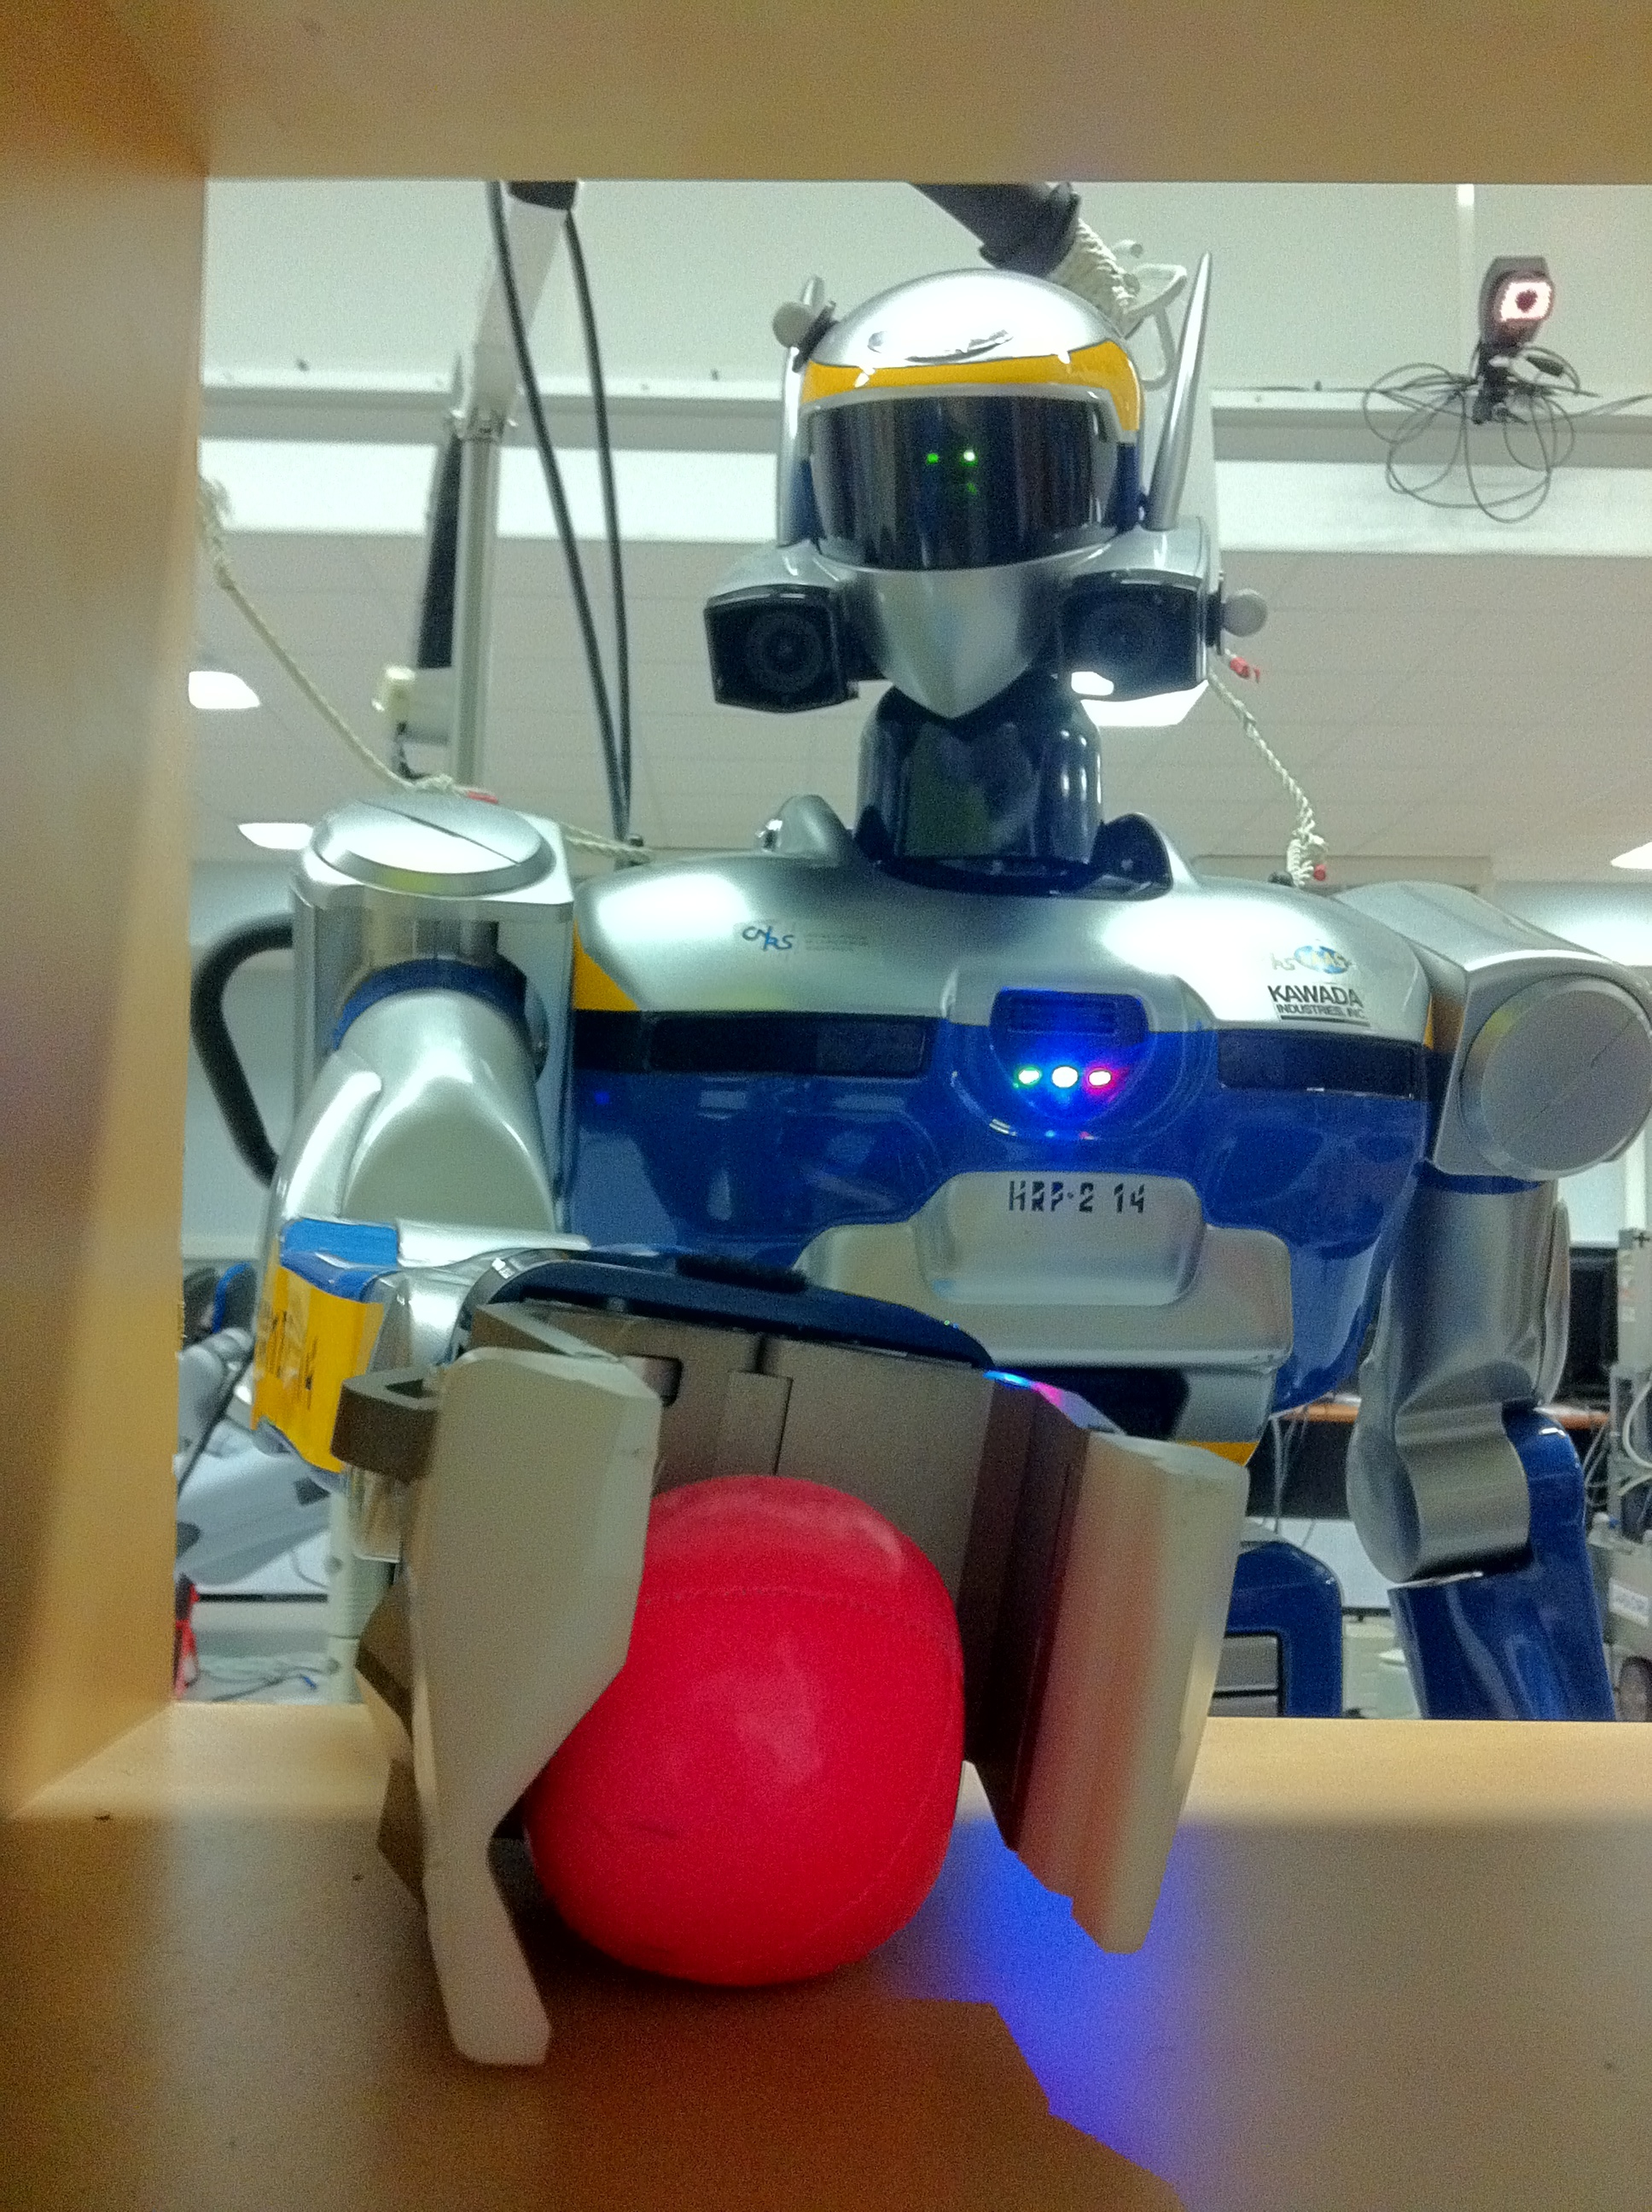
\includegraphics[width=\paperwidth,height=\paperheight]{%
      src/slides/demo1.jpg}}
  \begin{frame}[plain]
    \titlepage
  \end{frame}
}

%\maxFrameImage{src/slides/demo1.jpg}
%\maxFrameImage{src/slides/demo2.jpg}

% Introduction
% Animated scheme introducing contributions.
\begin{frame}
  \begin{changemargin}{-1cm}{-1cm}
    \begin{center}
      \tikzstyle{normalPath} = [line width=.7mm, color=black!50, -latex]

      \begin{tikzpicture}[
          auto,
          state/.style={
            rectangle,
            minimum size=6mm
          }]

        \uncover<1->{
          \node (perception) [state] {%
            
\includegraphics[height=3cm]{%
              src/slides/perception.pdf}};
        }

        \uncover<1>{
          \node (perception-description)
                [state, right=of perception]
                {\textbf{Perception}};
        }


        \uncover<2->{
          \node (decision)
               [state,above right=of perception] {%
            
\includegraphics[height=3cm]{%
              src/slides/decision.pdf}};
        }

        \uncover<2>{
          \node (decision-description)
                [state, right=of decision]
                {\textbf{Décision}};
        }

        \uncover<3->{
        \node (action) [state,below right=of decision]{%
          
\includegraphics[height=3cm]{%
            src/slides/action.pdf}};
        }

        \uncover<3>{
          \node (action-description)
                [state, left=of action]
                {\textbf{Action}};
        }

        \uncover<4->{
          \path (perception) edge[->, normalPath] (decision);
        }

        \uncover<5-8>{
          \path (decision) edge[->, normalPath] (action);
        }

        \uncover<6->{
          \path (action.south)
          edge[->, normalPath, dashed, bend right, bend left]
          node[color=black!50,above=5pt] {Monde réel}
          (perception.south);
        }

        \uncover<7->{
          \node (contrib) [state,left=of decision]{%
            \usebeamerfont{section}\large\textbf{Contributions}};

          \node (contrib1b) [state,right=1pt of decision]{%
            (1) RobOptim};
        }
        \uncover<7>{
          \node[thick,draw=ThoughfulBrick] (contrib1)
               [state,above=-3.4cm of decision] {%
                 \phantom{
\includegraphics[height=3.5cm]{%
                     src/slides/perception.pdf}}};
        }

        \uncover<8->{
          \path (perception.east)
          edge[->, normalPath,color=ThoughfulBrick]
          node[above=5pt] {(2) Correction}
          (action.west);
        }
        \uncover<8>{
          \node[thick,draw=ThoughfulBrick] (contrib2)
               [state,above=-3.4cm of action] {%
                 \phantom{
\includegraphics[height=3.5cm]{%
                     src/slides/action.pdf}}};
        }


        \uncover<9->{
          \path (decision) edge[->, normalPath,color=ThoughfulBrick]
          node[color=ThoughfulBrick,text width=3.5cm]{%
            (3) Primitives de mouvement} (action);
        }

        \uncover<10->{
          \node (contrib4b) [state,above=10pt of perception]{%
            (4) Intégration};
        }
        \uncover<10>{
          \node[thick,draw=ThoughfulBrick] (contrib4)
               [state,above=-3.4cm of perception] {%
                 \phantom{
\includegraphics[height=3.5cm]{%
                     src/slides/perception.jpg}}};
        }


      \end{tikzpicture}
    \end{center}
  \end{changemargin}
\end{frame}

\begin{slideDecision}
  \begin{changeleftmargin}{1.1cm}
    \frametitle{Processus de décision}
    \begin{center}
      \includegraphics%
          [width=.75\linewidth]%
          {src/chap1-roboptim/hrp2-two-chairs.png}

          \begin{enumerate}
          \item Planification.
          \item Optimisation de la trajectoire trouvée.
          \end{enumerate}
    \end{center}
  \end{changeleftmargin}
\end{slideDecision}

\begin{slideDecision}
  \begin{changeleftmargin}{1.1cm}
    \frametitle{Optimisation}
    \begin{equation*}
      \min_{\mathbf{x} \in \mathbb{R}^n} f(\mathbf{x})%
      \text{ sous la contrainte } \mathbf{x} \in \mathbf{X}
    \end{equation*}

    \begin{equation*}
      \mathbf{X} \equiv \left\{
      \begin{array}{l l}
        c_i (x) = 0    & \quad i \in \xi \\
        c_j (x) \leq 0 & \quad j \in \nu \\
      \end{array} \right.
    \end{equation*}

  \end{changeleftmargin}
\end{slideDecision}

\begin{slideDecision}
  \begin{changeleftmargin}{1.1cm}
    \frametitle{$\lambda$-calcul (1)}

    \begin{description}
      \item[Variables libres] $x$, $y$, \ldots
      \item[Application] $u v$ avec $u, v$ deux lambda-termes
      \item[Abstraction] $\lambda f x . t$ avec $x$ une variable, $t$
        un $\lambda$-terme.
    \end{description}
  \end{changeleftmargin}
\end{slideDecision}

\begin{slideDecision}
  \begin{changeleftmargin}{1.1cm}
    \frametitle{$\lambda$-calcul (2)}
    \begin{description}
      \item[Identité]~\\
        $\text{Id} \equiv \lambda x . x$
      \item[Entiers de Church]~\\
        $0 \equiv \lambda f x . x$\\
        $1 \equiv \lambda f x . f x$
      \item[Addition]~\\
        $\text{succ} \equiv \lambda n f x . f (n f x)$
    \end{description}
  \end{changeleftmargin}
\end{slideDecision}

\begin{slideDecision}
  \begin{changeleftmargin}{1.1cm}
    \frametitle{$\beta$-conversion}

    \begin{equation*}
      \begin{array}{ll}
      \text{succ}~1 & \rightarrow_\beta \lambda f x . (\lambda n f x . f (n f x)) (\lambda f x . f x)\\
        & \rightarrow_\beta \lambda f x . f ((\lambda f x . f x) f x)\\
        & \rightarrow_\beta \lambda f x . f f x \equiv 2\\
      \end{array}
    \end{equation*}

    \begin{center}
      \alert{réécrire $\equiv$ calculer $\equiv$ exécuter}
    \end{center}

  \end{changeleftmargin}
\end{slideDecision}

\begin{slideDecision}
  \begin{changeleftmargin}{1.1cm}
    \frametitle{$\lambda$-calcul simpement typé (1)}

    \begin{equation*}
      \Omega \equiv (\lambda x . x) (\lambda x . x)
    \end{equation*}

    \begin{equation*}
      (\lambda x . x) (\lambda x . x) \rightarrow_\beta
      (\lambda x . x) (\lambda x . x)
    \end{equation*}
  \end{changeleftmargin}
\end{slideDecision}

\begin{slideDecision}
  \begin{changeleftmargin}{1.1cm}
    \frametitle{$\lambda$-calcul simpement typé (2)}

    \begin{description}
    \item[Type naturel]~\\
      $x \vdash \iota$
    \item[Type fonctionnel]~\\
      $x \vdash \iota \wedge t \vdash \tau \Rightarrow \lambda x. t \vdash \iota \rightarrow \tau$
    \end{description}

    \bigskip

    $\Omega$ n'est pas correctement typé.

  \end{changeleftmargin}
\end{slideDecision}

\begin{slideDecision}
  \begin{changeleftmargin}{1.1cm}
    \frametitle{Programmation orientée objet (1)}

    \begin{equation*}
      A \equiv \{ \underbrace{\{ \text{foo} \vdash \iota
        \}}_{\mathfrak{A}}, \underbrace{\{ \text{bar} \vdash A
        \rightarrow \iota, \text{baz} \vdash A \rightarrow \iota
        \}}_{\mathfrak{M}} \}
    \end{equation*}

    \begin{equation*}
      a \vdash A \Rightarrow a.\text{foo} \vdash \iota
    \end{equation*}

    \begin{equation*}
      a \vdash A \Rightarrow a.\text{bar} \vdash A \rightarrow \iota
    \end{equation*}
  \end{changeleftmargin}
\end{slideDecision}

\begin{slideDecision}
  \begin{changeleftmargin}{1.1cm}
    \frametitle{Programmation orientée objet (2)}

    \begin{equation*}
      u v \text{bien formé} \Rightarrow u \vdash \tau_1 \rightarrow
      \tau_2 \wedge \tau_3 <: \tau_1
    \end{equation*}

    \begin{equation*}
      \tau_2 <: \tau_1 \Rightarrow
      \mathfrak{A_{\tau_1}} \subset \mathfrak{A_{\tau_2}} \wedge \mathfrak{M_{\tau_1}} \subset
      \mathfrak{M_{\tau_2}}
    \end{equation*}
  \end{changeleftmargin}
\end{slideDecision}

\begin{slideDecision}
  \begin{changeleftmargin}{1.1cm}
    \frametitle{Type paramétré}

    Fonction d'ordre supérieur $\text{type}
    \Rightarrow \text{type}$.

    \bigskip

    Exemple: $\tau_\alpha$
  \end{changeleftmargin}
\end{slideDecision}

\begin{slideDecision}
  \begin{changeleftmargin}{1.1cm}
    \frametitle{Représentation du problème (1)}

    \begin{equation*}
      \begin{array}{ll}
      \text{Fonction} \equiv & \{ \underbrace{\{ \#\text{entrée} \vdash
        \iota \}}_{\text{attributs}}, \\
      & \underbrace{\{ \text{calcule}
        \vdash \text{Fonction} \rightarrow[\iota] \rightarrow \iota \}}_{\text{méthode}} \}
      \end{array}
    \end{equation*}

    \begin{equation*}
      \begin{array}{l}
        \text{FonctionDérivable} \equiv \\
        \{ \{ \}, \{ \text{gradient}
      \vdash \text{FonctionDérivable} \rightarrow [\iota] \rightarrow [\iota] \} \}\\
      ~~<: \text{Fonction}
      \end{array}
    \end{equation*}

  \end{changeleftmargin}
\end{slideDecision}

\begin{slideDecision}
  \begin{changeleftmargin}{1.1cm}
    \frametitle{Représentation du problème (2)}

    \begin{equation*}
      \begin{array}{l}
        \text{Fonction}_n \equiv \text{Fonction} \quad \text{si $n = 0$}\\
        \text{Fonction}_n \equiv \text{FonctionDérivable} \quad \text{si $n = 1$}\\
        \text{Fonction}_n \equiv \\
        \{ \{ \}, \{ \text{gradient} \vdash \text{Fonction}_n \rightarrow \iota \rightarrow [\iota] \rightarrow [\iota] \} \}\\
        ~~<: \text{Fonction}_{n-1} \quad \text{si $n > 1$}\\
      \end{array}
    \end{equation*}

  \end{changeleftmargin}
\end{slideDecision}

\begin{slideDecision}
  \begin{changeleftmargin}{1.1cm}
    \frametitle{Représentation du problème (3)}

  \begin{equation*}
  \begin{split}
    \tau_{\text{prob}(\tau_1, \tau_2, \tau_3, \dotsc)} \equiv
    \{ \{ & \text{coût} \vdash \tau_1,\\
    & \text{contraintes} \vdash [\cup_{i \in \{2, \dotsc, n\}} \tau_i],\\
    & \text{bornes\_contraintes\_min} \vdash [\iota], \\
    & \text{bornes\_contraintes\_max} \vdash [\iota] \},\\
    & \{ \} \}\\
  \end{split}
  \end{equation*}

  \begin{equation*}
    \text{Solveur}_{\tau} \equiv \{ \{ \}, \{ \text{résous} \vdash
    \text{Solveur}_{\tau} \rightarrow \tau \rightarrow [\iota] \} \}
  \end{equation*}
  \end{changeleftmargin}
\end{slideDecision}

\begin{slideDecision}
  \begin{changeleftmargin}{1.1cm}
    \frametitle{Exemple: Optimisation non linéaire}

    \begin{description}
    \item[Fonction de coût]~\\
      $\text{Fonction}_2$
    \item[Contraintes linéaires]~\\
      $\text{FonctionLinéaire}$
    \item[Contraintes non linéaires]~\\
      $\text{Fonction}_2$
    \item[Problème]
    \end{description}

    ~~~~$\text{Problème}_{\text{prob}(\text{Fonction}_2, \text{FonctionLinéaire}, \text{Fonction}_2)}$

  \end{changeleftmargin}
\end{slideDecision}


\begin{slideDecision}
  \frametitle{RobOptim}
  \begin{changeleftmargin}{1.1cm}
  \begin{center}
    \tikzstyle{roboptim} = [align=center,
      rectangle,
      minimum size=6mm,
      minimum height=15mm,
      color=Thoughtless,
      fill=ThoughtBySome,
      line width=1pt,
      inner sep=0pt,
      outer sep=0pt,
      text width=70pt
    ]

    \begin{tabular}{cccl}
      \tikz \node[roboptim] (cfsqp) {CFSQP}; &
      \tikz \node[roboptim] (ipopt) {IPOPT}; &
      \tikz \node[roboptim] (others) {\ldots}; &
      \parbox[l][1.5cm][l]{2cm}{%
        \vspace{-.6cm}\rotatebox{-90}{\footnotesize \textbf{Solveur}}}\\
      \multicolumn{3}{c}{%
        \tikz \node[roboptim,
          text width=235pt] (core) {RobOptim Core};
      } &
      \parbox[l][1.5cm][l]{2cm}{%
        \vspace{-.6cm}\rotatebox{-90}{\footnotesize \textbf{Interface}}}\\
      \tikz \node[roboptim] (traj) {RobOptim Trajectory}; &
      \tikz \node[roboptim] (post) {RobOptim Posture}; &
      \tikz \node[roboptim] (others2) {\ldots}; &
      \parbox[l][1.5cm][l]{2cm}{%
        \vspace{-.6cm}\rotatebox{-90}{%
          \footnotesize \textbf{Application}}}\\
    \end{tabular}
  \end{center}
  \end{changeleftmargin}
\end{slideDecision}

\begin{slideDecision}
  \frametitle{Applications}

  \begin{center}
    \includegraphics[height=.33\paperheight]%
                    {src/chap1-roboptim/straight-line-obstacle.png}
  \includegraphics[height=.33\paperheight]%
                  {src/slides/agent-067.jpg}\par
  \includegraphics[height=.33\paperheight]%
                  {src/slides/multi-014.jpg}
  \includegraphics[height=.33\paperheight]%
                  {src/slides/multi-015.jpg}
%  \includegraphics[height=.33\paperheight]%
%                  {src/slides/deformable.jpg}

  Figures 2, 3, 4: K. Bouyarmane et collab.
  \end{center}
\end{slideDecision}


\begin{slideDecision}
  \frametitle{Génération de mouvements (1)}
  \begin{changeleftmargin}{1.1cm}
  \begin{center}
    
\includegraphics[width=.25\paperheight]{src/slides/falling.pdf}%
    
\includegraphics[width=.25\paperheight]{src/slides/burning.pdf}\par
    \bigskip
    Quelles contraintes?\par
  \end{center}
  Limites en torque et vitesse,\\
  (auto-)collision et \alert{équilibre}.
  \end{changeleftmargin}
\end{slideDecision}

\begin{slideDecision}
  \frametitle{Génération de mouvements (2)}
  \begin{changeleftmargin}{1.1cm}
    \begin{center}
      ZMP dans le polygone support $\Rightarrow$ mouvement
      dynamiquement stable.

      \bigskip

      \begin{tikzpicture}[%
          auto,
          footprint/.style={%
            rectangle,
            draw=black,
            ultra thick,
            minimum size=6mm,
            text width=8mm,
            decoration={brace},
        },
        fpLeft/.style={%
          footprint,
          decoration={brace, raise=-1.05cm},
        },
        fpRight/.style={%
          footprint,
          decoration={brace, raise=1.05cm},
        }]
        
        \matrix[ampersand replacement=\&,
          row sep=1cm, column sep=.5cm]{%
            \uncover<1-2>{
              \node[fpLeft] (l0) {};
            } \&
            \&
            \uncover<3->{
              \node[fpLeft] (l1) {};
            }\\
%           
            \uncover<1>{
              \node[fpRight] (r0) {};
            }\&
            \uncover<2-3>{
              \node[fpRight] (r1) {};
            } \&
            \&
            \uncover<4->{
              \node[fpRight] (r2) {};
            }\\
          };

        \path[draw,ultra thick]
        (l0.north west) -- (r0.south west);
        \path[draw,ultra thick]
        (l0.north west) -- (l0.north east);
        \path[draw,ultra thick]
        (r0.south west) -- (r0.south east);
        \path[draw,ultra thick]
        (l0.north east) -- (r0.south east);
      \end{tikzpicture}

    \end{center}
  \end{changeleftmargin}
\end{slideDecision}

\begin{slideDecision}
  \frametitle{Génération de mouvements (3)}
  \begin{changeleftmargin}{1.1cm}
  \begin{center}
    \begin{equation*}
    \begin{array}{lll}
    x_{ZMP} &=& x_G -
    \frac{\dot{\sigma}_y\ +\ m\ z_G\ \ddot{x}_G}{m\ (\ddot{z}_G + g)}\\
    y_{ZMP} &=& y_G +
    \frac{\dot{\sigma}_x - m z_G \ddot{y}_G}{m (\ddot{z}_G + g)}
    \end{array}
  \end{equation*}

  \end{center}

  \begin{description}
    \item[$(x_G, y_G, z_G)$]~\\
      Position du centre de masse.
    \item[$(\sigma_x, \sigma_y)$]~\\
      Moment autour du centre de masse.
    \item[$m$] Masse du robot.
    \item[$g$] Constante de gravité.
  \end{description}

  \end{changeleftmargin}
\end{slideDecision}

\begin{slideDecision}
  \frametitle{Génération de mouvements (4)}
  \begin{changeleftmargin}{1.1cm}
  \begin{center}

    Modèle linéaire:

    \begin{equation*}
      z = x - \frac{z_G}{g} \ddot{x}_G
    \end{equation*}

    \begin{description}
    \item[$z$] Position du ZMP.
    \item[$x$] Position du centre de masse.
    \item[$z_G$] Hauteur du centre de masse.
    \item[$g$] Constante de gravité.
    \end{description}
  \end{center}
  \end{changeleftmargin}
\end{slideDecision}

\begin{slideDecision}
  \frametitle{Génération de mouvements (5)}
  \begin{changeleftmargin}{1.5cm}
  \begin{center}
    \begin{enumerate}
      \item Génération d'une pile de pas.
      \item Génération d'une trajectoire de ZMP.
      \item Génération de la trajectoire de centre de masse
        correspondante.
      \item Génération des trajectoires de pieds.
    \end{enumerate}

    \bigskip

    \alert{Et la trajectoire corps complet?}
  \end{center}
  \end{changeleftmargin}
\end{slideDecision}

\maxFrameImageWidth{src/chap3-primitive-mouvement/footsteps1.jpg}

\begin{slideAction}
  \frametitle{Contrôleur polyvalent (1)}

  \begin{changeleftmargin}{1.1cm}
  \begin{center}
    Contrôleur: algorithme générant la commande envoyée aux moteurs à
    une fréquence fixe (200Hz pour HRP-2).

    \bigskip

    \begin{itemize}
    \item Exécute les mouvements générés par la partie décisionelle.
    \item En charge de l'adaptation réactive du mouvement.
    \item Respecte le temps réel.
    \end{itemize}

    \bigskip

    Composant \alert{critique} de tout robot.
  \end{center}
  \end{changeleftmargin}
\end{slideAction}

\begin{slideAction}
  \frametitle{Contrôleur polyvalent (2)}

  \begin{changeleftmargin}{1.1cm}
  \begin{center}
    Espace des tâches\\
    VS\\
    Espaces des configurations.

    \bigskip

    \begin{equation*}
      \mathbf{e} = \mathbf{s} - \mathbf{s}^{*}
    \end{equation*}

    \begin{description}
      \item[$\mathbf{e}$] erreur.
      \item[$\mathbf{s}$] valeur courante de la tâche.
      \item[$\mathbf{s}^{*}$] valeur de référence.
    \end{description}
  \end{center}
  \end{changeleftmargin}
\end{slideAction}

\begin{slideAction}
  \frametitle{Contrôleur polyvalent (2)}

  \begin{changeleftmargin}{1.1cm}
  \begin{center}

    \begin{tikzpicture}[%
        >=latex,
        node distance=1em,
        fixed/.style={
          text width=120pt}]
      \node [state,fixed] (com) {Centre de masse};
      \node [state,fixed, below=of com] (lf) {Pied gauche};
      \node [state,fixed, below=of lf] (rf) {Pied droit};
      \node [state,fixed, below=of rf] (posture) {Posture};

      \node [left=of com] (fort) {Priorité forte};
      \node [left=of posture] (faible) {Priorité faible};
      \draw[->, line width=1.05]
      (fort.south) -- (faible.north);
    \end{tikzpicture}
  \end{center}
  \end{changeleftmargin}
\end{slideAction}

\begin{slideAction}
  \frametitle{Schéma de contrôle boucle fermée}

  \begin{center}
    \begin{tikzpicture}[>=latex]

      \draw (-1,-2) node [state] (ctrl) {Contrôleur};

      \draw (-1,0) node [state] (corr) {Correction};
      \draw (-1,1.5) node [state] (gen) {Génération};

      \draw (4,0) node (loc) [state] {Localisation};

      \draw[-,style=dashed] (2,-3) -- (2,3);

      \uncover<3-> {
        \draw[->] (loc.west) -- (corr.east)
        node [at start,left,font=\tiny,yshift=0.2cm]
        {$\hat{\mathbf{x}}_t \in \text{SE}(2)$};
      }

      \uncover<2-> {
        \draw[->] (gen.south) -- (corr.north)
        node [at start,left,font=\tiny,yshift=-0.2cm]
        {$(\gamma_{\text{pieds}}(t), \gamma_{\text{com}}(t), \mathbf{x}(t)) \in \text{SE}(3)^3 \times \text{SE}(2)$};
      }

      \uncover<3-> {
        \draw[->] (corr.south) -- (ctrl.north)
        node [at start,left,font=\tiny,yshift=-0.25cm]
        {$(\gamma'_{\text{pied~gauche}}(t), \gamma'_{\text{pied~droit}}(t), \gamma'_{\text{com}}(t)) \in \text{SE}(3)^3$};
      }

      \uncover<4-> {
        \draw[->] (ctrl.south) --++ (0,-1)
        node [at start,left,font=\tiny,yshift=-0.25cm]
        {$\dot{\mathbf{q}}_t \in \mathbb{R}^n$};
      }

      \draw[<-] (gen.north) --++ (0,1) node [left,font=\tiny,yshift=-0.25cm]
           {$\mathbf{S} \in \text{SE}(2)^{\text{nsteps}}$};
    \end{tikzpicture}
  \end{center}
\end{slideAction}

\begin{slideAction}
  \frametitle{Synchronisation temporelle}


  \begin{center}
    \vspace{-1cm}
    \begin{tikzpicture}
      \begin{axis}[
          grid=major,
          legend style={
            at={(0.5,-0.2)},
            anchor=north,
            legend columns=3,
            cells={anchor=west},
            font=\footnotesize,
            rounded corners=2pt,
            draw=white
          },
          xlabel=time ($s$),
          ylabel=$x$ position ($m$),
          no markers
          ]

        \addplot[
          red,
          dashed,
        ] table {dat/feet_follower_feet-follower-com.dat};
        \addlegendentry{center of mass}

        \addplot[
          blue,
          dashed,
        ] table[
          x index=0,
          y index=4
        ] {dat/feet_follower_feet-follower-left-ankle.dat};
        \addlegendentry{left foot}

        \addplot[
          green,
          dashed,
        ] table[
          x index=0,
          y index=4
        ] {dat/feet_follower_feet-follower-right-ankle.dat};
        \addlegendentry{right foot}

        \uncover<7->{
        \addplot[
          red,
        ] table {dat/feet_follower_correction-com.dat};
        \addlegendentry{center of mass (corr.)}
        }

        \uncover<6->{
        \addplot[
          blue,
        ] table[
          x index=0,
          y index=4
        ] {dat/feet_follower_correction-left-ankle.dat};
        \addlegendentry{left foot (corr.)}
        }

        \uncover<5->{
        \addplot[
          green,
        ] table[
          x index=0,
          y index=4
        ] {dat/feet_follower_correction-right-ankle.dat};
        \addlegendentry{right foot (corr.)}
        }
      \end{axis}

      \uncover<2-> {
        \draw [
        thick,
        decoration={
          brace,
          raise=-1.05cm
        },
        font=\tiny,
        decorate
      ] (axis cs:2.1,6.35) -- (axis cs:4.1,6.35)
      node [pos=0.5,anchor=north,yshift=-0.55cm] {pas 1};
      }

      \uncover<3-> {
      \draw [
        thick,
        decoration={
          brace,
          raise=-1.05cm
        },
        font=\tiny,
        decorate
      ] (axis cs:5.1,6.35) -- (axis cs:7.1,6.35)
      node [pos=0.5,anchor=north,yshift=-0.55cm] {pas 2};
      }

      % error measure
      \uncover<4-> {
      \draw[<-]
      (1.3, 0.5) -- (1.3, 1.5)
      node [font=\tiny,anchor=north,yshift=0.3cm, line width=1.3]
      {mesure};
      }

      \def\w{0.5}
      \def\h{0.75}
      \def\dx{8.}

      \def\dy{.5}
      % left step planned 1
      \filldraw[pattern=north east lines] (\dx + 0., \dy + 0.5)
      rectangle (\dx + 0. + \w, \dy + \h + 0.5);

      % left step planned 1 - drift
      \uncover<4-> {
        \draw[style=solid,color=red,line width=1.25] (\dx, \dy - 0.3 + 0.5)
        rectangle (\dx + \w, \dy + \h - 0.3 + 0.5);
      }

      \filldraw[pattern=north east lines] (\dx + 1., \dy + 0.5)
      rectangle (\dx + 1. + \w, \dy + \h + 0.5);
      \draw<4->[style=solid,color=red,line width=1.25] (\dx + 1., \dy - 0.3 + 0.5)
      rectangle (\dx + \w + 1., \dy + \h - 0.3 + 0.5);


      % right step planned 1
      \filldraw[pattern=north east lines] (\dx + 1., \dy + 3.)
      rectangle (\dx + 1. + \w, \dy + \h + 3.)
      node [pos=0.5,anchor=north,font=\tiny,yshift=0.75cm] {pas 1};

      % right step planned 1 - corrected
      \uncover<4-> {
        \draw[style=solid,color=red,line width=1.25]
        (\dx + 1., \dy + 3.-0.3)
        rectangle (\dx + 1. + \w, \dy + \h + 3. -0.3);
      }


      \uncover<5-> {
        \draw[style=solid,color=green,line width=1.25] (\dx + 1., \dy + 3.)
        rectangle (\dx + 1. + \w, \dy + \h + 3.);
      }

      \def\dy{3.}
      % left step planned 2
      \filldraw[pattern=north east lines] (\dx + 0., \dy + 0.5)
      rectangle (\dx + 0. + \w, \dy + \h + 0.5)
      node [pos=0.5,anchor=north,font=\tiny,yshift=0.75cm] {pas 2};

      \uncover<4-> {
        \draw[style=solid,color=red,line width=1.25] (\dx, \dy + 0.5 -0.3)
        rectangle (\dx + \w, \dy + \h + 0.5 -0.3);
      }

      % left step planned 2 - corrected
      \uncover<6-> {
        \draw[style=solid,color=green,line width=1.25] (\dx + 0., \dy + 0.5)
      rectangle (\dx + 0. + \w, \dy + \h + 0.5);
      }

    \end{tikzpicture}
  \end{center}
\end{slideAction}

\begin{slideAction}
  \frametitle{Trajectoire des pieds (1)}

  \begin{center}
    \begin{tikzpicture}[>=latex]
        \def\w{0.5}
        \def\h{0.75}

        \foreach \dy in {0., 1., 2., 3.}
                 {
                   % left step planned
                   \filldraw[pattern=north east lines] (0., \dy)
                   rectangle (0. + \w, \dy + \h);

                   % right step planned
                   \filldraw[pattern=north west lines] (1., \dy + 0.5)
                   rectangle (1. + \w, \dy + \h + 0.5);
                 }

        % before correction
        \def\driftx{0.1}
        \def\drifty{0.05}
        \def\drifttheta{5.}

        \def\dy{0}
        % left step planned
        \draw<2->[style=solid, color=red, rotate=\drifttheta * \dy,line width=1.25]
        (0. + \driftx * \dy, \drifty * \dy + \dy)
        rectangle (0. + \driftx * \dy + \w, \drifty * \dy + \dy + \h);

        % right step planned
        \draw<3->[style=solid, color=red, rotate=\drifttheta * \dy + \drifttheta / 2.,line width=1.25]
        (1. + \driftx * \dy + \drifty / 2., \drifty * \dy + \drifty / 2. + \dy + 0.5)
        rectangle (1. + \driftx * \dy + \drifty / 2. + \w, \drifty * \dy + \drifty / 2. + \dy + \h + 0.5);

        \def\dy{1}
        % left step planned
        \draw<4->[style=solid, color=red, rotate=\drifttheta * \dy,line width=1.25]
        (0. + \driftx * \dy, \drifty * \dy + \dy)
        rectangle (0. + \driftx * \dy + \w, \drifty * \dy + \dy + \h);

        % right step planned
        \draw<5->[style=solid, color=red, rotate=\drifttheta * \dy + \drifttheta / 2.,line width=1.25]
        (1. + \driftx * \dy + \drifty / 2., \drifty * \dy + \drifty / 2. + \dy + 0.5)
        rectangle (1. + \driftx * \dy + \drifty / 2. + \w, \drifty * \dy + \drifty / 2. + \dy + \h + 0.5);


        \def\dy{2}
        \draw<6->[style=solid, color=red,line width=1.25, rotate=\drifttheta] (0. + \driftx, \dy + \drifty)
        rectangle (0. + \w + \driftx, \dy + \h + \drifty);

        % --- after correction ---

        % left step planned
        \draw<7->[style=solid, color=green,line width=1.25] (0., \dy)
        rectangle (0. + \w, \dy + \h);

        \uncover<7->{
        \draw[smooth,rounded corners=1ex,<-,thick]
        (-0.3, \dy) -- (-0.3 - 0.05, \dy + 0.2) -- (-0.3 - 0.2, \dy + 0.4)
        node[midway,left]
        {
          $\delta \mathbf{x}$
        };
        }


        \draw<7->[style=solid, color=green,line width=1.25] (0., \dy)
        rectangle (0. + \w, \dy + \h);
        \draw<7->[style=solid, color=green,line width=1.25] (1., \dy + 0.5)
        rectangle (1. + \w, \dy + \h + 0.5);
        \def\dy{3}
        \draw<7->[style=solid, color=green,line width=1.25] (0., \dy)
        rectangle (0. + \w, \dy + \h);
        \draw<7->[style=solid, color=green,line width=1.25] (1., \dy + 0.5)
        rectangle (1. + \w, \dy + \h + 0.5);

        % right step planned
        \def\dy{2}
        \draw<8->[style=solid, color=orange,line width=1.25, rotate=\drifttheta * 0.5] (1. + \driftx * .5, \dy + 0.5 + \drifty * 0.5)
        rectangle (1. + \driftx * 0.5 + \w, \dy + \drifty * 0.5 + \h + 0.5);

        \def\dy{3}
        % left step planned
        \draw<9->[style=solid, color=orange,line width=1.25, rotate=\drifttheta * 1.] (0. + \driftx * 1., \dy + \drifty * 1.)
        rectangle (0. + \w + \driftx * 1., \dy + \h + \drifty * 1.);

        % right step planned
        \uncover<10-> {
          \draw[style=solid, color=orange,line width=1.25, rotate=\drifttheta * 1.5] (1. + \driftx * 1.5, \dy + 0.5 + \drifty * 1.5)
        rectangle (1. + \w + \driftx * 1.5, \dy + \h + 0.5 + \drifty * 1.5);
        }

      \end{tikzpicture}
      \end{center}
\end{slideAction}

\begin{slideAction}
  \frametitle{Trajectoire des pieds (2)}

  \begin{equation*}
    \gamma_{\text{pied}}^{(1)}(t) = \Delta^t(t) . \gamma_{\text{pied}}(t)
  \end{equation*}

  \begin{equation*}
    \gamma_{\text{foot}}^{(n)}(t) =
    ( \prod_{i=0}^{n-1}\Delta^{t_{n-i}}(t) ) . \gamma_{\text{pied}}(t)
  \end{equation*}

\end{slideAction}

\begin{slideAction}
  \frametitle{Trajectoire du centre de masse}

  \begin{equation*}
    \mathbf{z} = \mathbf{c} - \frac{z_c}{g} \ddot{\mathbf{c}}
  \end{equation*}

  \begin{equation*}
    \mathbf{c}^{(n)}(t) =
    \underbrace{\scriptstyle \cosh(\sqrt{\frac{g}{z_c}}.t) . \mathbf{V} +
      \sinh(\sqrt{\frac{g}{z_c}}.t) . \mathbf{W} +
      \mathbf{r}(t)}_{\mathbf{c}(t) \in \mathbb{R}^2} + \sum_{i=1}^n \Delta^{t_i}(t)
  \end{equation*}

  \begin{center}
    $\mathbf{V}$, $\mathbf{W}$ déterminent la position et vitesse
    initiale.
  \end{center}

  \begin{equation*}
    \forall t \in \mathbb{R}, \Delta^t(0) = \dot{\Delta}^t(0) = 0
  \end{equation*}
\end{slideAction}

\maxFrameImageHeight{src/chap2-suivi-trajectoire/demo.jpg}


%\maxFrameImageHeight{src/chap3-primitive-mouvement/calibextrinsic.jpg}

\begin{slidePerception}
  \frametitle{Systèmes de localisation}

  \begin{changeleftmargin}{1.1cm}
  \begin{description}
  \item[Capture de mouvement] Précision $\pm 1$ cm. Environnement
    instrumenté.
  \item[Tracker] Algorithme de vision. Précision à quelques
    centimètres près. Méthode locale.
  \item[Odométrie visuelle] Précision trop faible.
  \end{description}
  \end{changeleftmargin}
\end{slidePerception}

\maxFrameImageHeight{src/chap4-integration/shelf.png}

\begin{frame}
  \frametitle{Conclusion}

  \begin{itemize}
  \item Architecture complète: perception, décision, action.
  \item Correction des pas pour les mouvements de précision.
  \end{itemize}

  \bigskip

  \begin{itemize}
  \item Valider l'approche pour les bras.
  \item Valider les pas corrigés en-ligne.
  \item Améliorer la localisation du robot. Utilisation conjointe de
    plusieurs systèmes de localisation.
  \end{itemize}
\end{frame}

\maxFrameImageHeight{src/slides/hrp2-thx.jpg}


%
%\begin{slidePerception}
%  \frametitle{De la bibliothèque au composant}
%
%  FIXME
%\end{slidePerception}

%\maxFrameImageHeight{src/slides/demo2.jpg}

%\maxFrameImageHeight{src/chap4-integration/footsteps2.jpg}
%\maxFrameImageHeight{src/chap4-integration/disparity-1.jpg}
%\maxFrameImageHeight{src/chap4-integration/disparity-2.jpg}
%\maxFrameImageHeight{src/chap4-integration/hrp2_urdf.jpg}
%\maxFrameImageHeight{src/chap4-integration/rviz-full.jpg}



\end{document}
